\documentclass[12pt, a4paper]{article}
\setlength{\headheight}{20pt}
%\renewcommand{\baselinestretch}{1.5}
\usepackage[margin=3cm]{geometry}
\usepackage{setspace}
\onehalfspacing
%\usepackage{mathptmx}% Times Roman font
%\usepackage{utopia}
%\usepackage{newcomputermodern}
\usepackage{lmodern}
\usepackage{amsmath}
\usepackage{amssymb}
\usepackage{mdframed}
\usepackage[T1]{fontenc}
\usepackage{fancyhdr}
\usepackage{pgfplots}
\newcommand\s{30} %samples i grafer. set til 1000, 80 for arbejde
%\newcommand{\doubleunderline}{\underline{\underline{}}}
\usepackage{lipsum}
\usepackage{blindtext}
%flyta myndir
\usepackage{graphicx}
\usepackage{float}
\usepackage{sidecap}
%flyta myndir end

\usepackage{titlesec}
\titleformat{\section}
{\Large \bfseries}
{\thesection}
{1em}
{}

\titleformat{\subsection}
{\large}
{\thesubsection}
{0.5em}
{}

%bruka inkscapefílir
\usepackage{import}
\usepackage{xifthen}
\usepackage{pdfpages}
\usepackage{transparent}

\newcommand{\incfig}[1]{%
    \def\svgwidth{6.00cm}
    \import{./figures/}{#1.pdf_tex}
}
\renewcommand*\contentsname{Indholdsfortegnelse}
%bruka inkscapefílir end

\usepackage[backend=biber,sorting=nty,style=verbose]{biblatex}
\addbibresource{bibliografi.bib} %Imports bibliography file
\DeclarePrintbibliographyDefaults{heading=none}
\title{Taylorpolynomier}
%\author{Jákup H. Lützen}
\date{Februar 2022}
%\pagestyle{fancy}
%\fancyhead{}
%\fancyfoot{}
\begin{document}
\begin{titlepage}
   \centering
    \vfill
%    \maketitle
    {\huge 
    Taylorpolynomier\\
    \vspace{0.5cm}
    \large
    SSO\\
    \vspace{0.25cm}
    Februar 2022
    }    
    \vfill
%    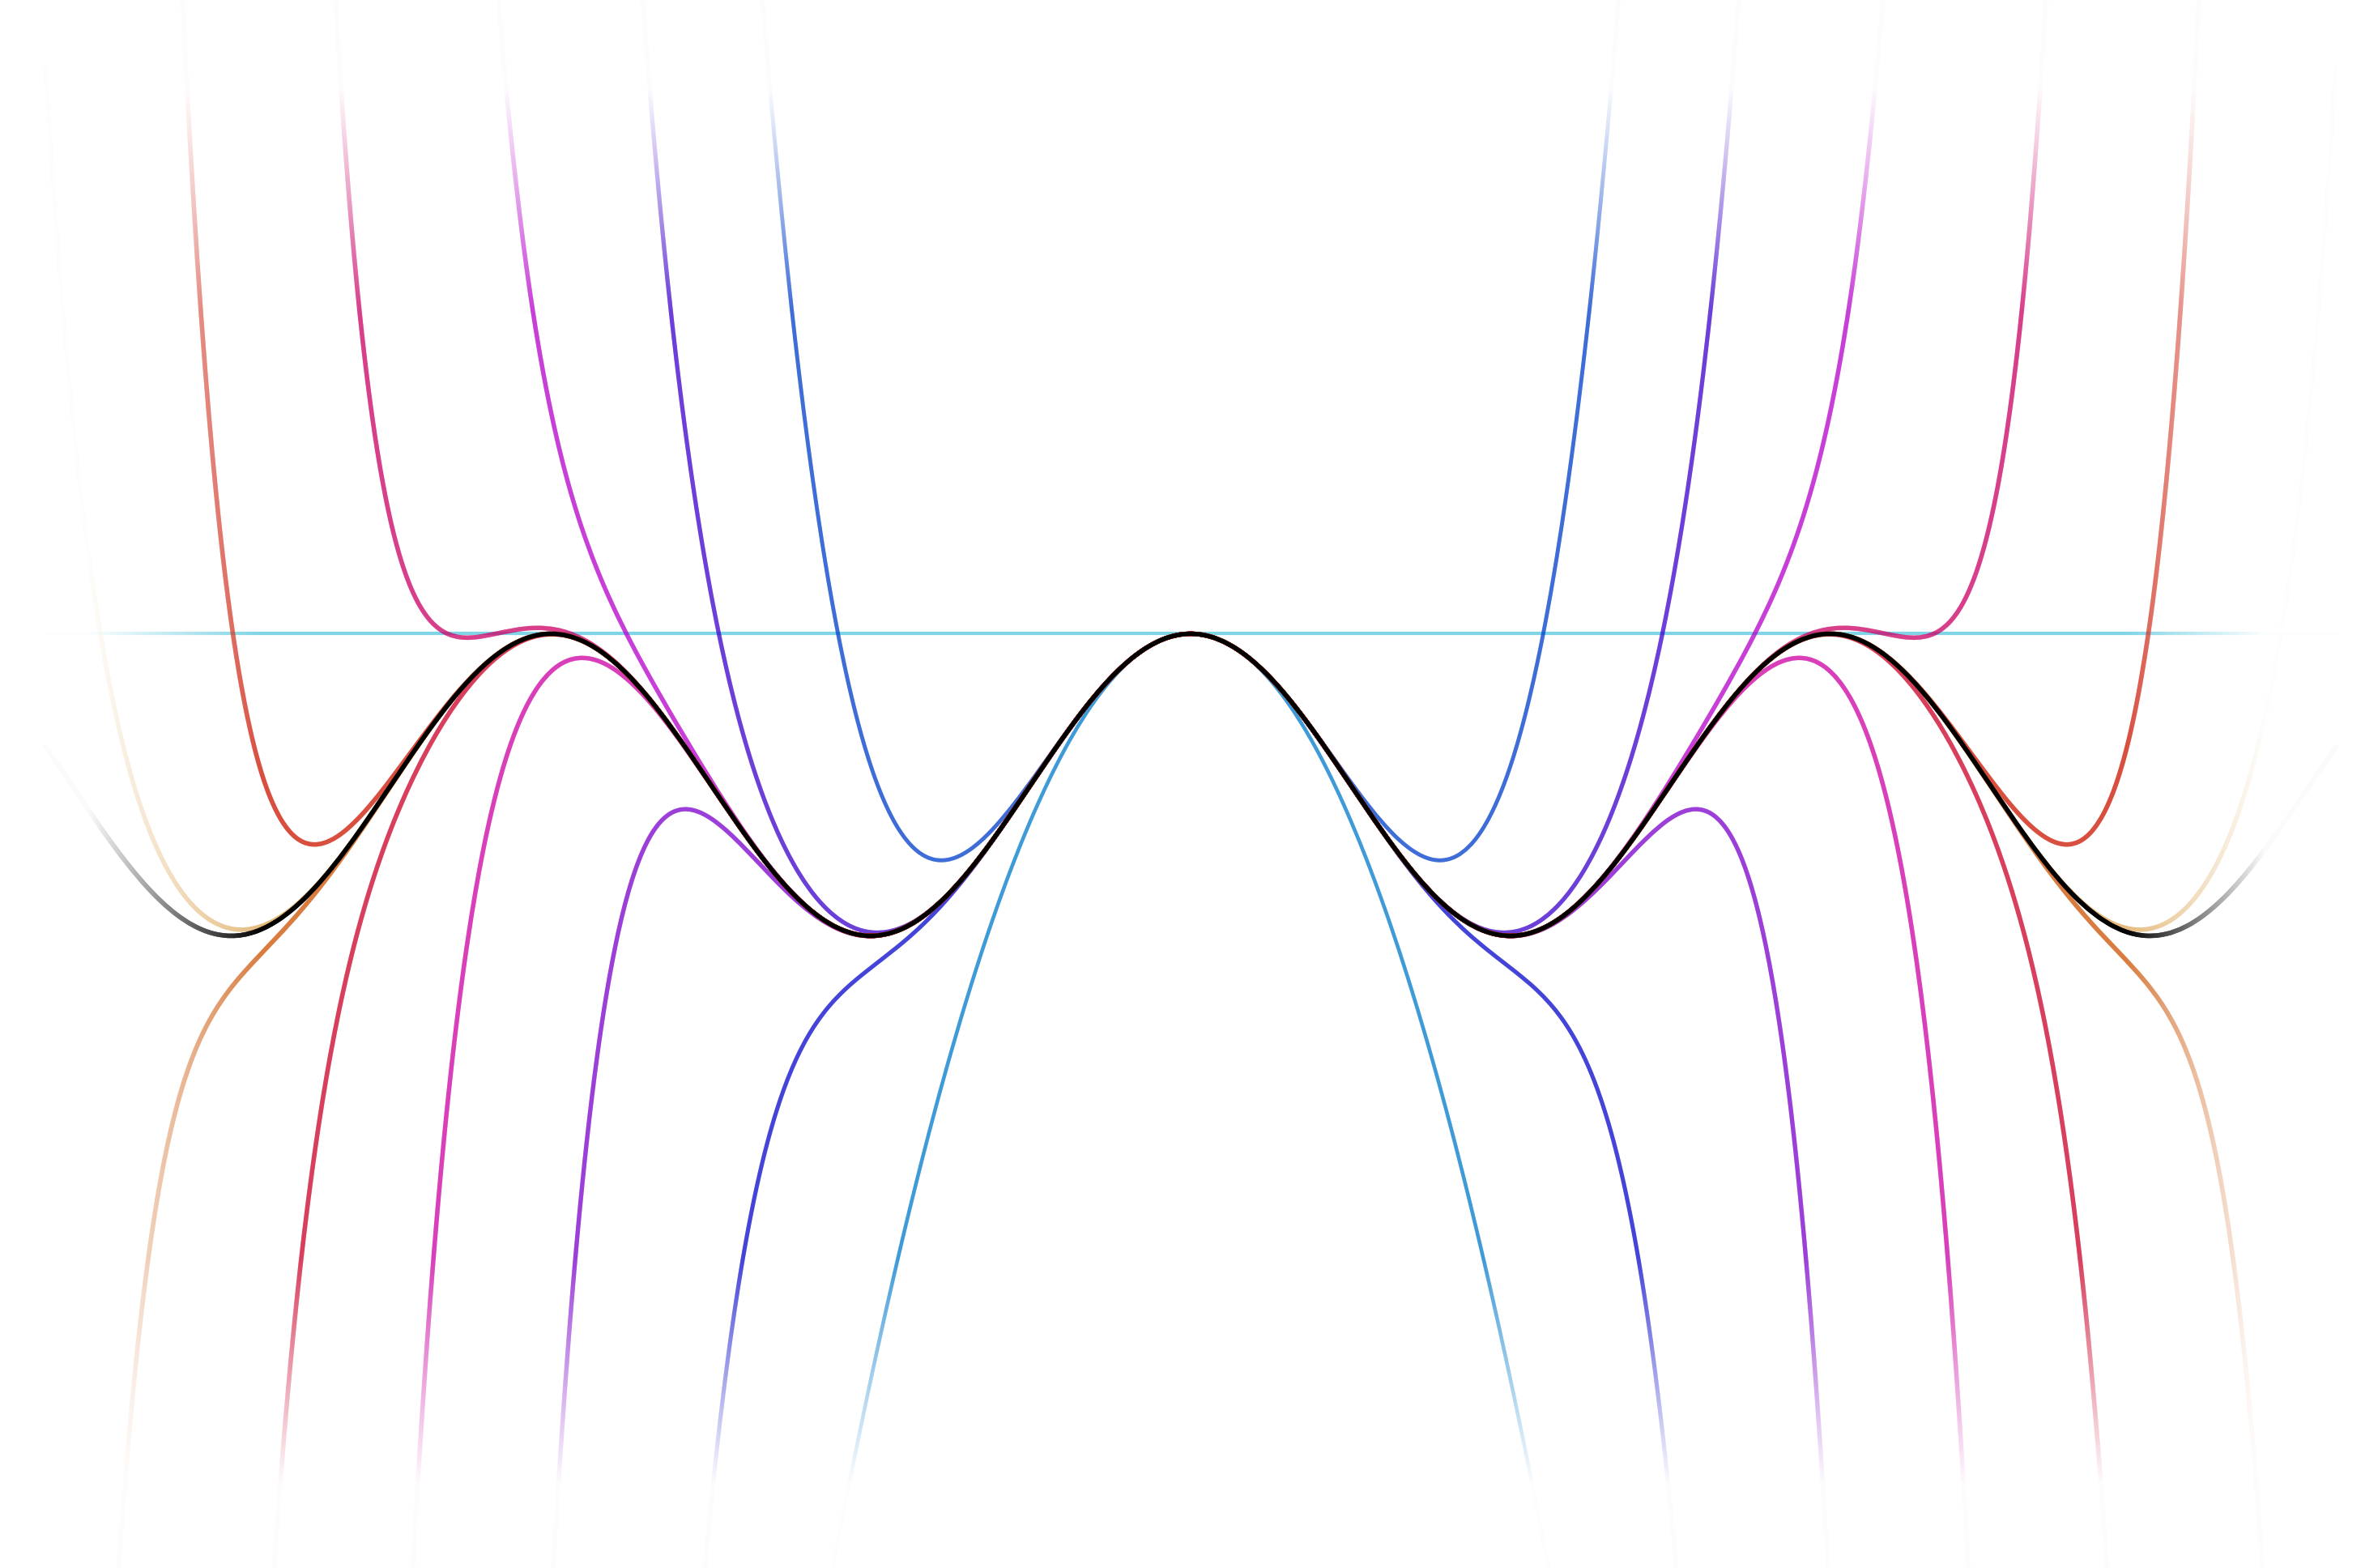
\includegraphics[width=\textwidth]{figures/forside3edit2.png} % also works with logo.pdf
   
    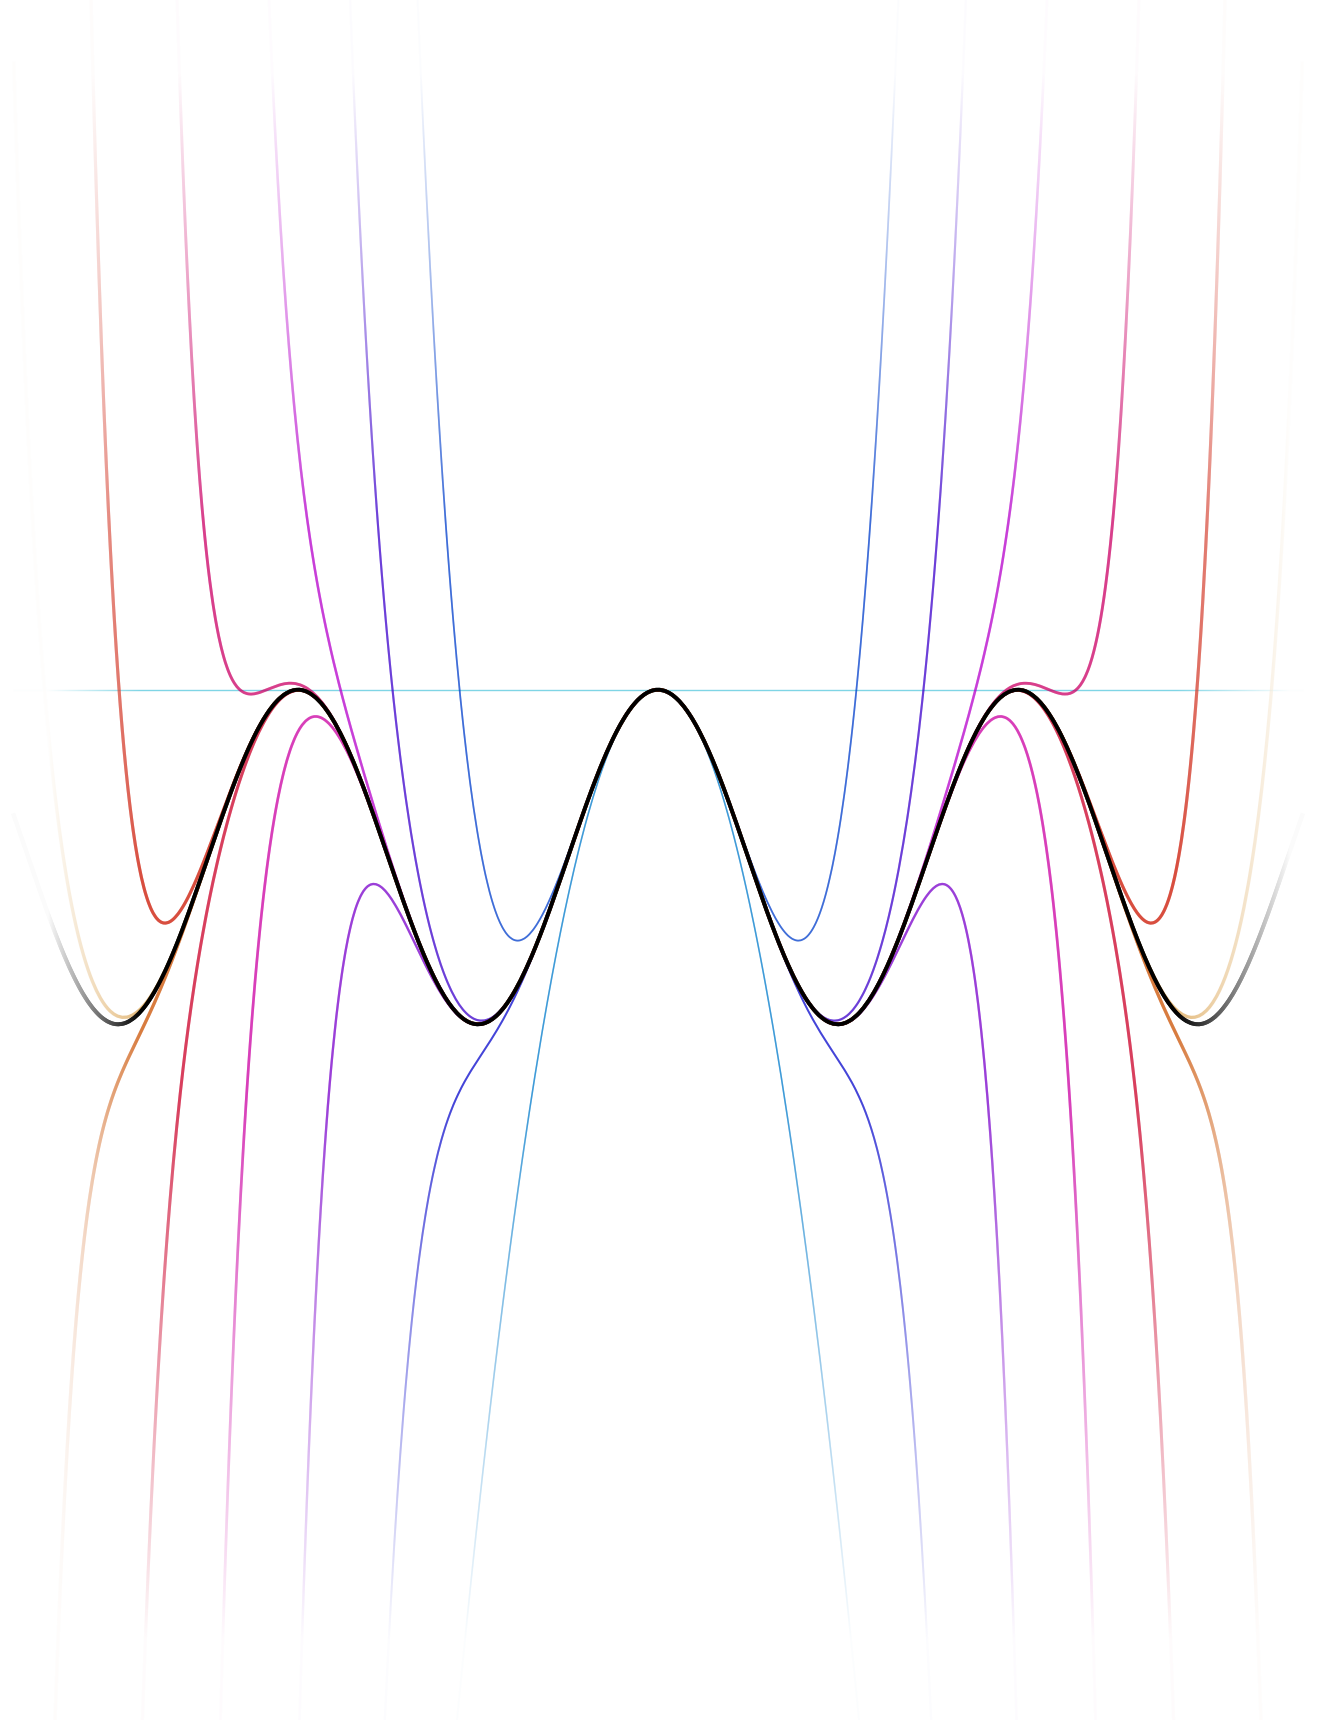
\includegraphics[width=\textwidth]{figures/forside4edit.png} % also works with logo.pdf
    \vfill
    \vfill
\thispagestyle{empty}

\end{titlepage}
%%%%% \footnote{hey} fyri vanligan footnote
%%%%%\footcite{talogrækker} fyri referencu
%%%%% :set spell spelllang=da (fyri at byrja spellcheck)
%%%% :set nospell fyri at sløkkja
\section*{Resume} %150 ord (det essentielle i min opgave, dvs ca 8 linjer
\blindtext[1-2]
\tableofcontents
\newpage



\section{Indledning} %ca en halv side til en side. I egne ord, hvorfor dette er interessant. God ide at slutte af med problemformuleringen, "Og her vil jeg..."
lMatematik kan synes firkantet og rigidt, hvor abstrakte forhold opskrives i eksakte formler, og hvor der ikke er plads til kreativitet. Dykker man dybere ind i faget vil man dog opdage, at dette ikke er tilfældet, og at der er mange situationer, hvor man gør kreativt brug af ueksakte værktøjer. Et af disse er såkaldte Taylorpolynomier.


I \underline{matematikkens} \footcite{uvm} verden findes der alverdens slags funktioner, hvor nogle er mere medgørlige end andre.\\
\\
Jeg vil i denne opgave redegøre for hvad et Taylorpolynomium er, undersøge Taylorpolynomier i et historisk lys, samt undersøge hvilke praktiske anvendelser de kan have.

\section{Redegørelse} % Egne ord. Ikke inddrage citater (fordi så bliver det analyserende).

\section{Analyse} % Kød og kartofler. Brug modellen (introducere citatet, så kommer citatet, og så kommenterer man.

\section{Diskussion/Vurdering} % Måske tage nogle fagpersoner med eller noget. Gerne selv tage stilling.


\section{Konklusion} % samle problemformuleringens underspørgsmål. "jeg har. og så... jeg kan konkludere..."

\section{Litteraturliste}
\nocite{*}
\subsection{Fysiske materialer:}
\printbibliography[keyword=bøger]
\subsection{Onlinematerialer:}
\printbibliography[keyword=online]
Forsidebillede er skabt af undertegnede.
\end{document}

